\documentclass[../main.tex]{subfiles}

\begin{document}
\chapter{Liniowo przekształcony rozkład kosinusowy}
\label{Chapter:LTC}

Do rozwiązania całki w równaniu renderingu można podejść w zupełnie inny sposób. Dla świateł powierzchniowych autorzy \cite{ltc_heitz} zaproponowali znalezienie przybliżenie wyrażenia całkowego na sferze następującej postaci:
\[
L_o(\omega_o) = \int_{P} {
  L_i(\omega_i)
  f_r(\omega_i, \omega_o)
  \cos \theta_i
  \dd \omega_i
}
\approx
\int_{P} {
  L_i(\omega_i)
  D(\omega_i)
  \dd \omega_i
}
\]

\noindent gdzie $P$ jest wielokątem reprezentującym światło obszarowe rzutowanym na sferę jednostkową. Innymi słowy, $P$ wyznacza wszystkie kierunki promieni przecinających powierzchnię światła, a $D(\omega)$ jest naszą szukaną funkcją aproksymującą.

Funkcję $D(\omega)$ \footnote{Funkcja $D(\omega)$ nie jest związana z z funkcją rozkładu normalnych, oznaczenie zostało zachowane dla kompatybilności z pracą \cite{ltc_heitz}.} chcielibyśmy dobrać tak, aby całe wyrażenie posiadało wzór jawny lub było możliwe do przybliżenia w bardzo krótkim czasie.

Autorzy pracy \cite{ltc_heitz} postanowili najpierw uprościć problem jeszcze bardziej i znaleźć taki rozkład, który można całkować niezależnie w czasie rzeczywistym i pozwala modelować  zjawiska istotne dla funkcji BRDF. Chcielibyśmy, aby dla danego rozkładu $D(\omega)$ całka poniższej postaci była możliwa do obliczenia:
\[
\int_P {
    D(\omega)
    \dd \omega
}
\]

Zakładając znajomość rozwiązania powyższej całki, takie uproszczenie pozwala nam na proste rozwiązanie całki dla światła o jednorodnym kolorze tzn. dla przypadku, w którym, gdy dowolny promień $\omega$ przecina $P$ to $L(\omega)=L$:
\[
\int_{P} {
    L_i(\omega_i)
    D(\omega_i)
    \dd \omega_i
} = \int_{P} {
    L *
    D(\omega_i)
    \dd \omega_i
} = L \int_{P} {
    D(\omega_i)
    \dd \omega_i
}
\]

\section{Wybór rozkładu $D(\omega)$}

Rozpocznijmy od zdefiniowania warunków, które funkcja $D(\omega)$ musi spełniać, aby nadawała się do zastosowania jako element przybliżenia. W zaawansowanych modelach oświetlenia bazowanych na zjawiskach fizycznych występuje kilka ważnych efektów, które muszą zostać zachowane. Również, ze względu na różnorodność materiałów występujących w typowej scenie metoda musi wspierać zmienną chropowatość powierzchni określoną przez parametr $\alpha$.

Pierwszym z istotnych efektów jest odpowiedź funkcji BRDF dla powierzchni obserwowanych pod odpowiednio dużym kątem. Odpowiedź powierzchni zostaje rozciągnięta wzdłuż jednej z osi formując kształt eliptyczny (rys. \ref{fig:BRDFGrazingAnisotropy}).

\begin{figure}
    \centering
    
    \begin{subfigure}[t]{0.18\textwidth}
        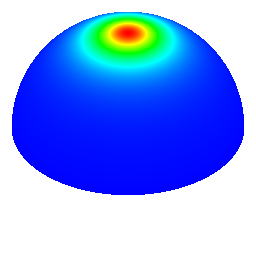
\includegraphics[width=\textwidth]{ltc/fit_r28_a0_brdf}
    \end{subfigure}
    \begin{subfigure}[t]{0.18\textwidth}
        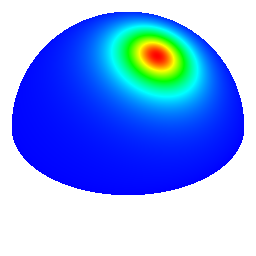
\includegraphics[width=\textwidth]{ltc/fit_r28_a16_brdf}
    \end{subfigure}
    \begin{subfigure}[t]{0.18\textwidth}
        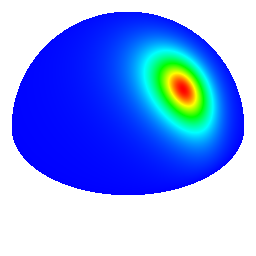
\includegraphics[width=\textwidth]{ltc/fit_r28_a32_brdf}
    \end{subfigure}
    \begin{subfigure}[t]{0.18\textwidth}
        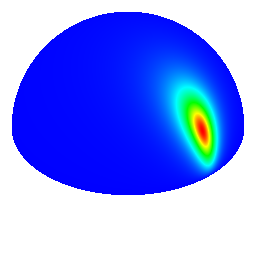
\includegraphics[width=\textwidth]{ltc/fit_r28_a48_brdf}
    \end{subfigure}
    \begin{subfigure}[t]{0.18\textwidth}
        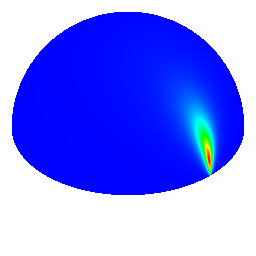
\includegraphics[width=\textwidth]{ltc/fit_r28_a60_brdf}
    \end{subfigure}
    
    \caption{Zjawisko rozciągnięcia odpowiedzi BRDF na jednej osi przy dużym kącie padania wiązki. Do wygnerowania podglądu wykorzystano model GGX. Opracowanie własne.}
    \label{fig:BRDFGrazingAnisotropy}
\end{figure}

Drugim jest to, że w takiej samej sytuacji zwiększając chropowatość materiału rozkład będzie się rozszerzał i deformował skośnie powodując, że jest on bardziej rozproszony bliżej normalnej (rys. \ref{fig:BRDFOffSpecular}). Powyższe zjawisko jest znane jako maksimum poza kątem odbicia (ang. \textit{off-specular peak}).

\begin{figure}
    \centering
    
    \begin{subfigure}[t]{0.18\textwidth}
        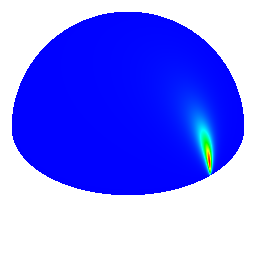
\includegraphics[width=\textwidth]{ltc/offspecular/fit_r25_a60_brdf}
    \end{subfigure}
    \begin{subfigure}[t]{0.18\textwidth}
        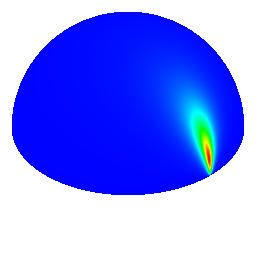
\includegraphics[width=\textwidth]{ltc/offspecular/fit_r30_a60_brdf}
    \end{subfigure}
    \begin{subfigure}[t]{0.18\textwidth}
        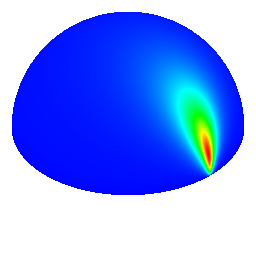
\includegraphics[width=\textwidth]{ltc/offspecular/fit_r35_a60_brdf}
    \end{subfigure}
    \begin{subfigure}[t]{0.18\textwidth}
        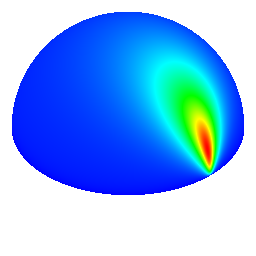
\includegraphics[width=\textwidth]{ltc/offspecular/fit_r40_a60_brdf}
    \end{subfigure}
    \begin{subfigure}[t]{0.18\textwidth}
        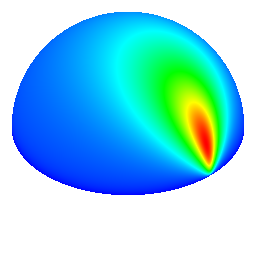
\includegraphics[width=\textwidth]{ltc/offspecular/fit_r45_a60_brdf}
    \end{subfigure}
    
    \caption{Zjawisko przesuwania się maksimum w kierunku normalnej. Do wygnerowania podglądu wykorzystano model GGX. Opracowanie własne.}
    \label{fig:BRDFOffSpecular}
\end{figure}

%\begin{figure}
%    \centering
%    
%    \begin{subfigure}[t]{0.3\textwidth}
%        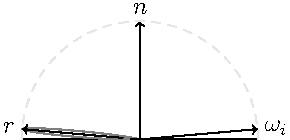
\includegraphics[width=\textwidth]{ltc/offspecular_0}
%        \caption{\ang{5} nachylenia, $\alpha = 0.2^2$}
%    \end{subfigure}
%    \begin{subfigure}[t]{0.3\textwidth}
%        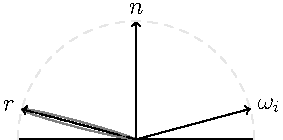
\includegraphics[width=\textwidth]{ltc/offspecular_1}
%        \caption{\ang{15} nachylenia, $\alpha = 0.2^2$}
%    \end{subfigure}
%    \begin{subfigure}[t]{0.3\textwidth}
%        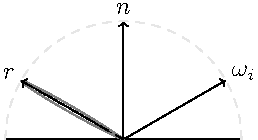
\includegraphics[width=\textwidth]{ltc/offspecular_2}
%        \caption{\ang{30} nachylenia, $\alpha = 0.2^2$}
%    \end{subfigure}
%
%    \begin{subfigure}[t]{0.3\textwidth}
%        \centering
%        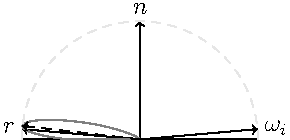
\includegraphics[width=\textwidth]{ltc/offspecular_3}
%        \caption{\ang{5} nachylenia, $\alpha = 0.4^2$}
%    \end{subfigure}
%    \begin{subfigure}[t]{0.3\textwidth}
%        \centering
%        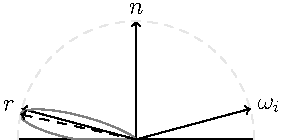
\includegraphics[width=\textwidth]{ltc/offspecular_4}
%        \caption{\ang{15} nachylenia, $\alpha = 0.4^2$}
%    \end{subfigure}
%    \begin{subfigure}[t]{0.3\textwidth}
%        \centering
%        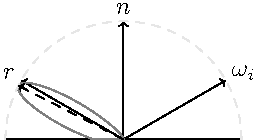
\includegraphics[width=\textwidth]{ltc/offspecular_5}
%        \caption{\ang{30} nachylenia, $\alpha = 0.4^2$}
%    \end{subfigure}
%
%    \begin{subfigure}[t]{0.3\textwidth}
%        \centering
%        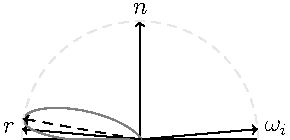
\includegraphics[width=\textwidth]{ltc/offspecular_6}
%        \caption{\ang{5} nachylenia, $\alpha = 0.6^2$}
%    \end{subfigure}
%    \begin{subfigure}[t]{0.3\textwidth}
%        \centering
%        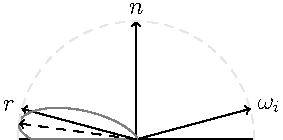
\includegraphics[width=\textwidth]{ltc/offspecular_7}
%        \caption{\ang{15} nachylenia, $\alpha = 0.6^2$}
%    \end{subfigure}
%    \begin{subfigure}[t]{0.3\textwidth}
%        \centering
%        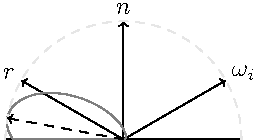
\includegraphics[width=\textwidth]{ltc/offspecular_8}
%        \caption{\ang{30} nachylenia, $\alpha = 0.6^2$}
%    \end{subfigure}
%
%    \begin{subfigure}[t]{0.3\textwidth}
%        \centering
%        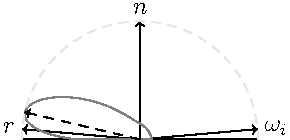
\includegraphics[width=\textwidth]{ltc/offspecular_9}
%        \caption{\ang{5} nachylenia, $\alpha = 0.8^2$}
%    \end{subfigure}
%    \begin{subfigure}[t]{0.3\textwidth}
%        \centering
%        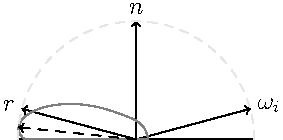
\includegraphics[width=\textwidth]{ltc/offspecular_10}
%        \caption{\ang{15} nachylenia, $\alpha = 0.8^2$}
%    \end{subfigure}
%    \begin{subfigure}[t]{0.3\textwidth}
%        \centering
%        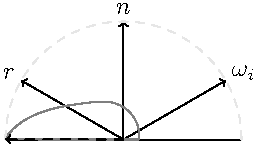
\includegraphics[width=\textwidth]{ltc/offspecular_11}
%        \caption{\ang{30} nachylenia, $\alpha = 0.8^2$}
%    \end{subfigure}
%    
%    \caption{Różnice między najsilniejszym kierunkiem odbicia od powierzchni o chropowatości $\sqrt{\alpha}$, a kierunkiem odbicia idealnego $r$. Do wygenerowania wykorzystano model GGX. Opracowanie własne.}
%    \label{fig:BRDFOffSpecular}
%\end{figure}

Warto zauważyć, że gdy $D$ jest rozkładem gęstości prawdopodobieństwa to całka:
\[
\int_P {
    D(\omega)
    \dd \omega
}
\]
\noindent definiuje całkowite prawdopodobieństwo, że próbka wygenerowana z rozkładu $D$ przetnie wielokąt $P$.

Najprostszą, już wcześniej wspomnianą metodą nie nadającą się do zastosowań czasu rzeczywistego jest metoda Monte-Carlo polegająca na wielokrotnym wybraniu losowego wektora z rozkładu $D$ i sprawdzenia istnienia punktu przecięcia tego promienia z wielokątem. Dla odpowiednio dużej liczby próbek stosunek trafień do ilości przetestowanych promieni będzie przybliżał naszą szukaną całkę.

Kluczową obserwacją jest to, że rozkład jest równoważny nieskończonej ilości próbek tego rozkładu. Każdą z tych form da się przekształcić na drugą w sposób bezpośredni i bezstratny. Zatem rozkład na sferze jest obiektem dualnym do nieskończonego zbioru ilości próbek tego samego rozkładu \cite{ltc_heitz}. Wynika z tego to, że po zmodyfikowaniu jednego otrzymamy nowy obiekt matematyczny.

Przykładem takiej operacji może być przekształcenie liniowe modyfikujące kierunek próbki (zakładać będziemy, że próbka po przekształceniu liniowym w dalszym ciągu jest jednostkowej długości tzn. zawsze zostaje z powrotem znormalizowana). Takie przekształcenie ma kilka bardzo ważnych właściwości, które będziemy wykorzystywać. Warto zauważyć, że jeżeli przekształcimy rozkład prawdopodobieństwa przekształceniem $M$ to gdy zrobimy to samo z wielokątem $P$ otrzymując wielokąt $P'$, to prawdopodobieństwo, że nowa próbka przetnie nowy wielokąt się nie zmieni – widać to wyraźnie z faktu, że przekształcone próbki podążają za przekształcanym wielokątem. Wynika stąd, że:
\[
\int_P {
  D(\omega)
  d \omega
} = \int_{P'} {
  D'(\omega)
  d\omega
}
\]

\begin{figure}
    \centering
    \begin{subfigure}[t]{0.45\textwidth}
        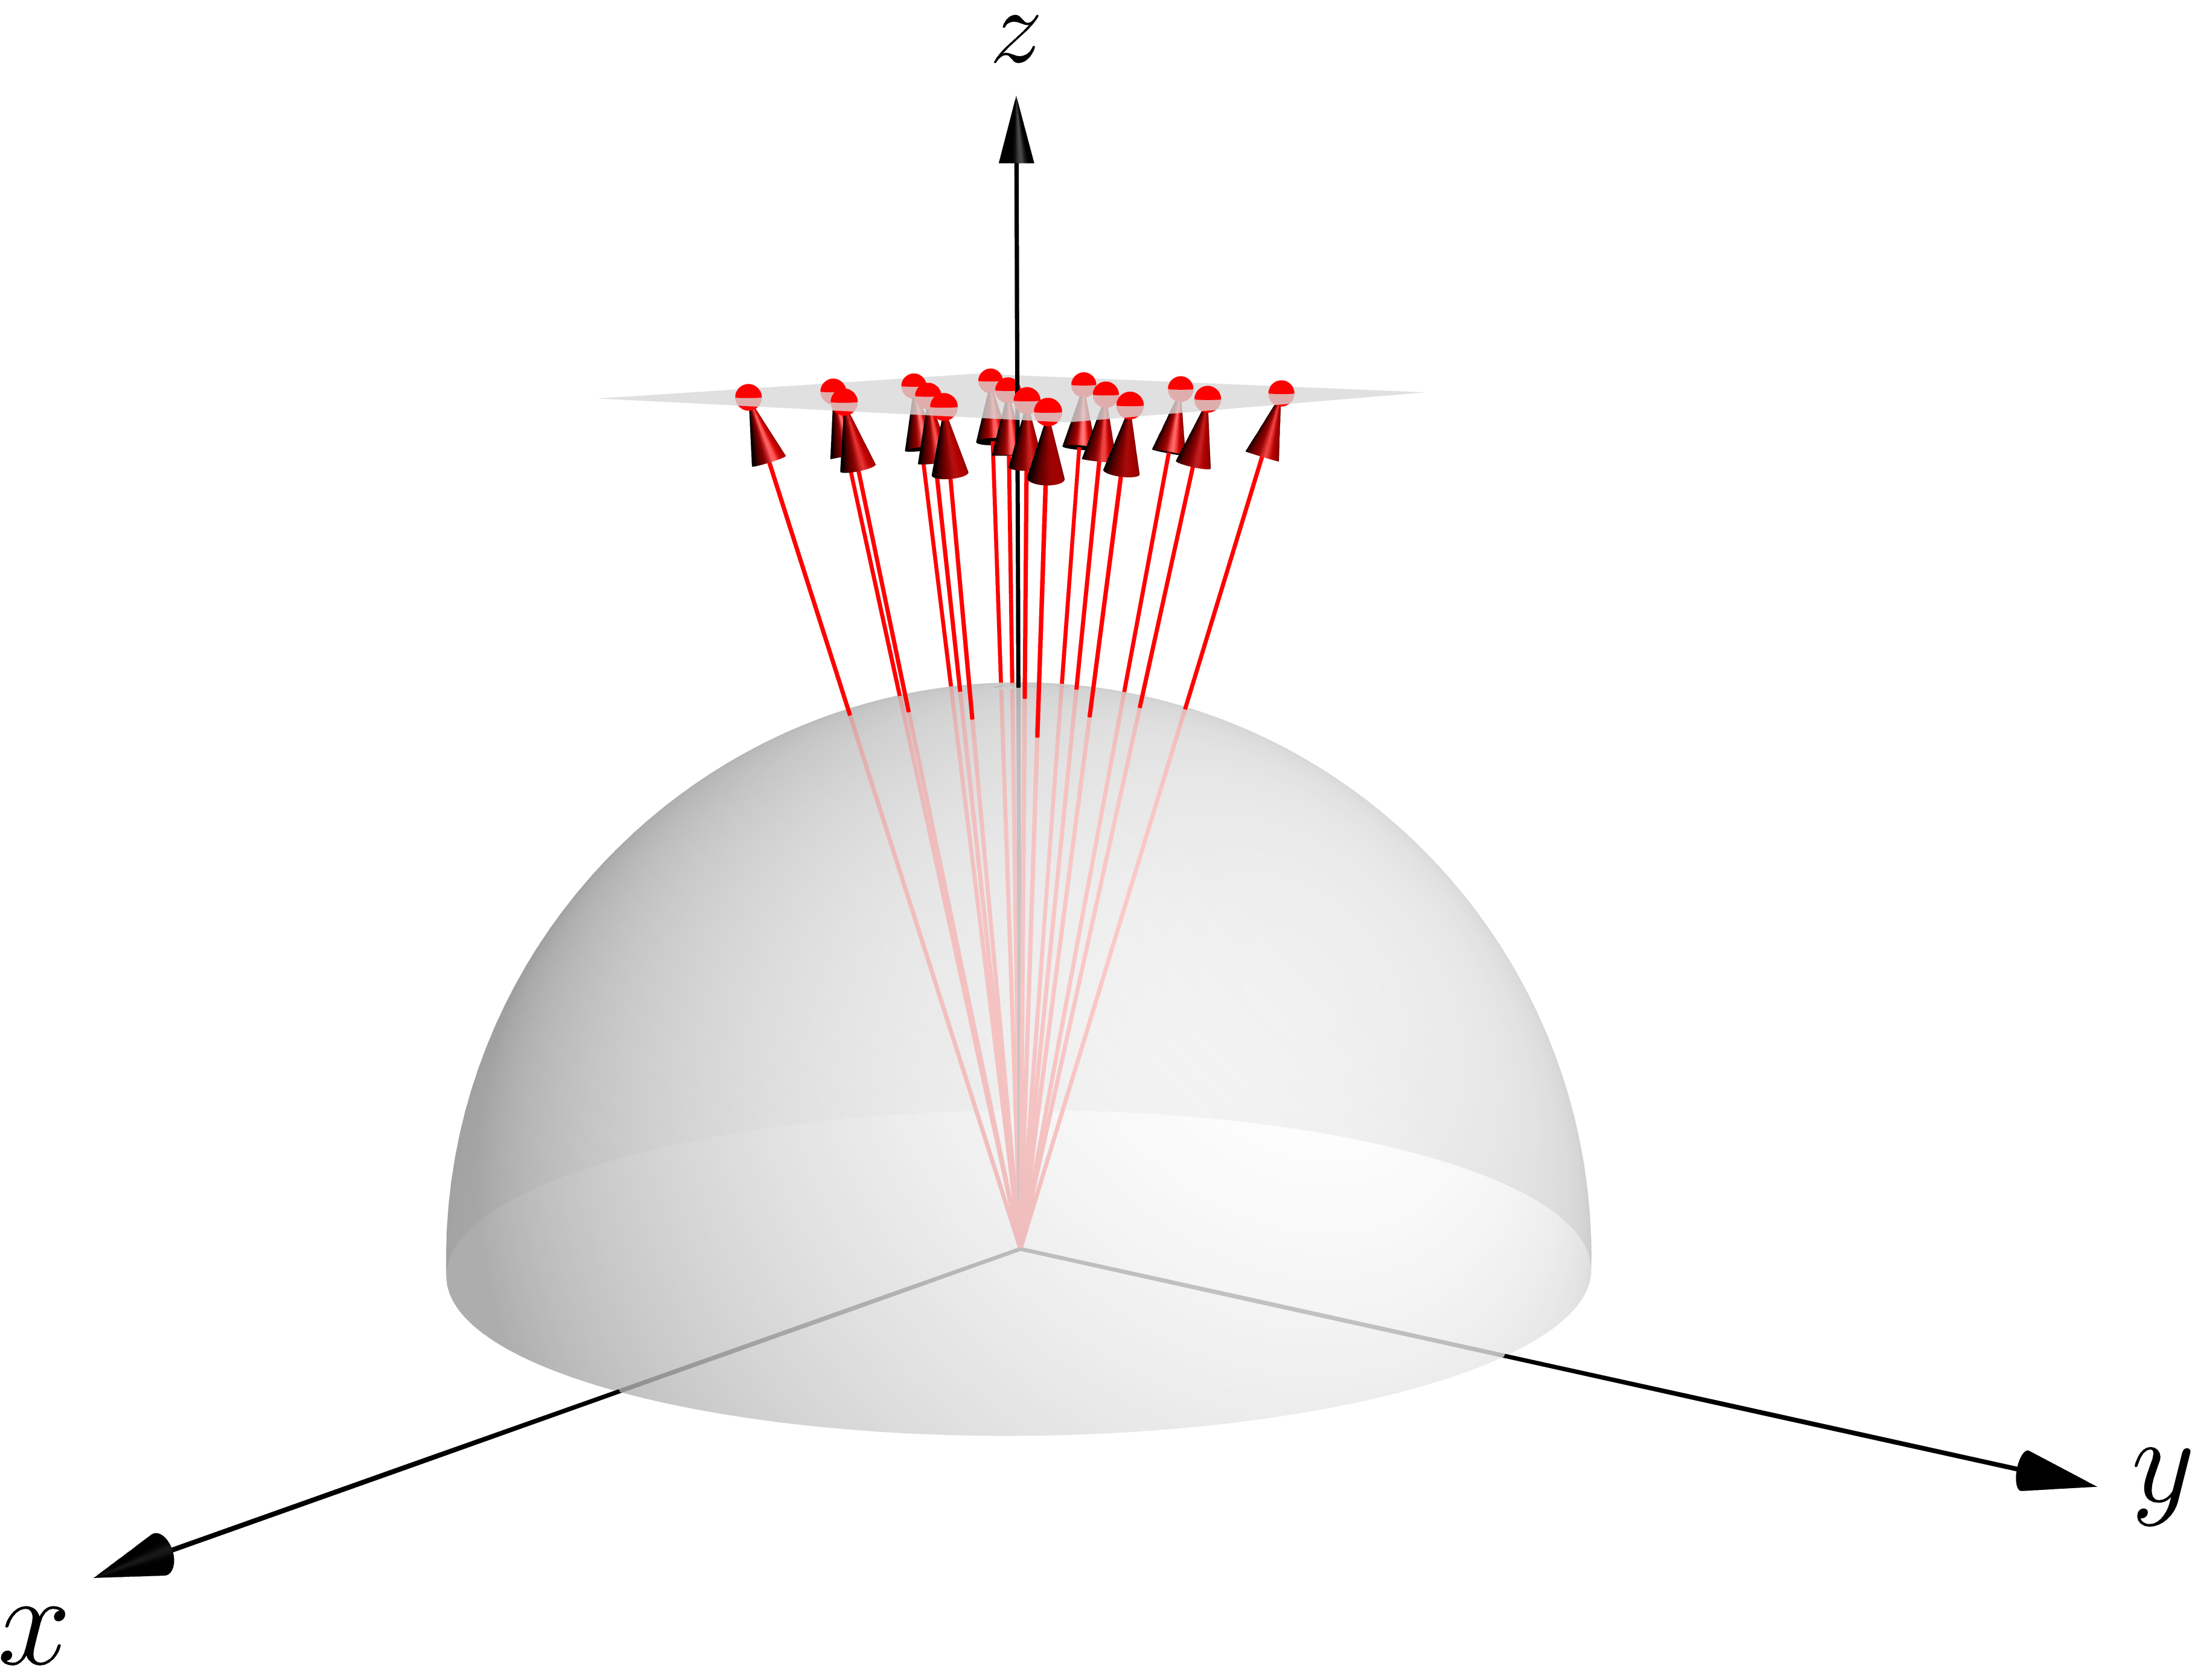
\includegraphics[width=\textwidth]{ltc/sample_transform_before}
        \label{fig:LTCTransformBefore}
        \caption{Nieprzekształcone promienie oraz wielokąt $P$}
    \end{subfigure}
    \hspace{0.05\textwidth}
    \begin{subfigure}[t]{0.45\textwidth}
        \centering
        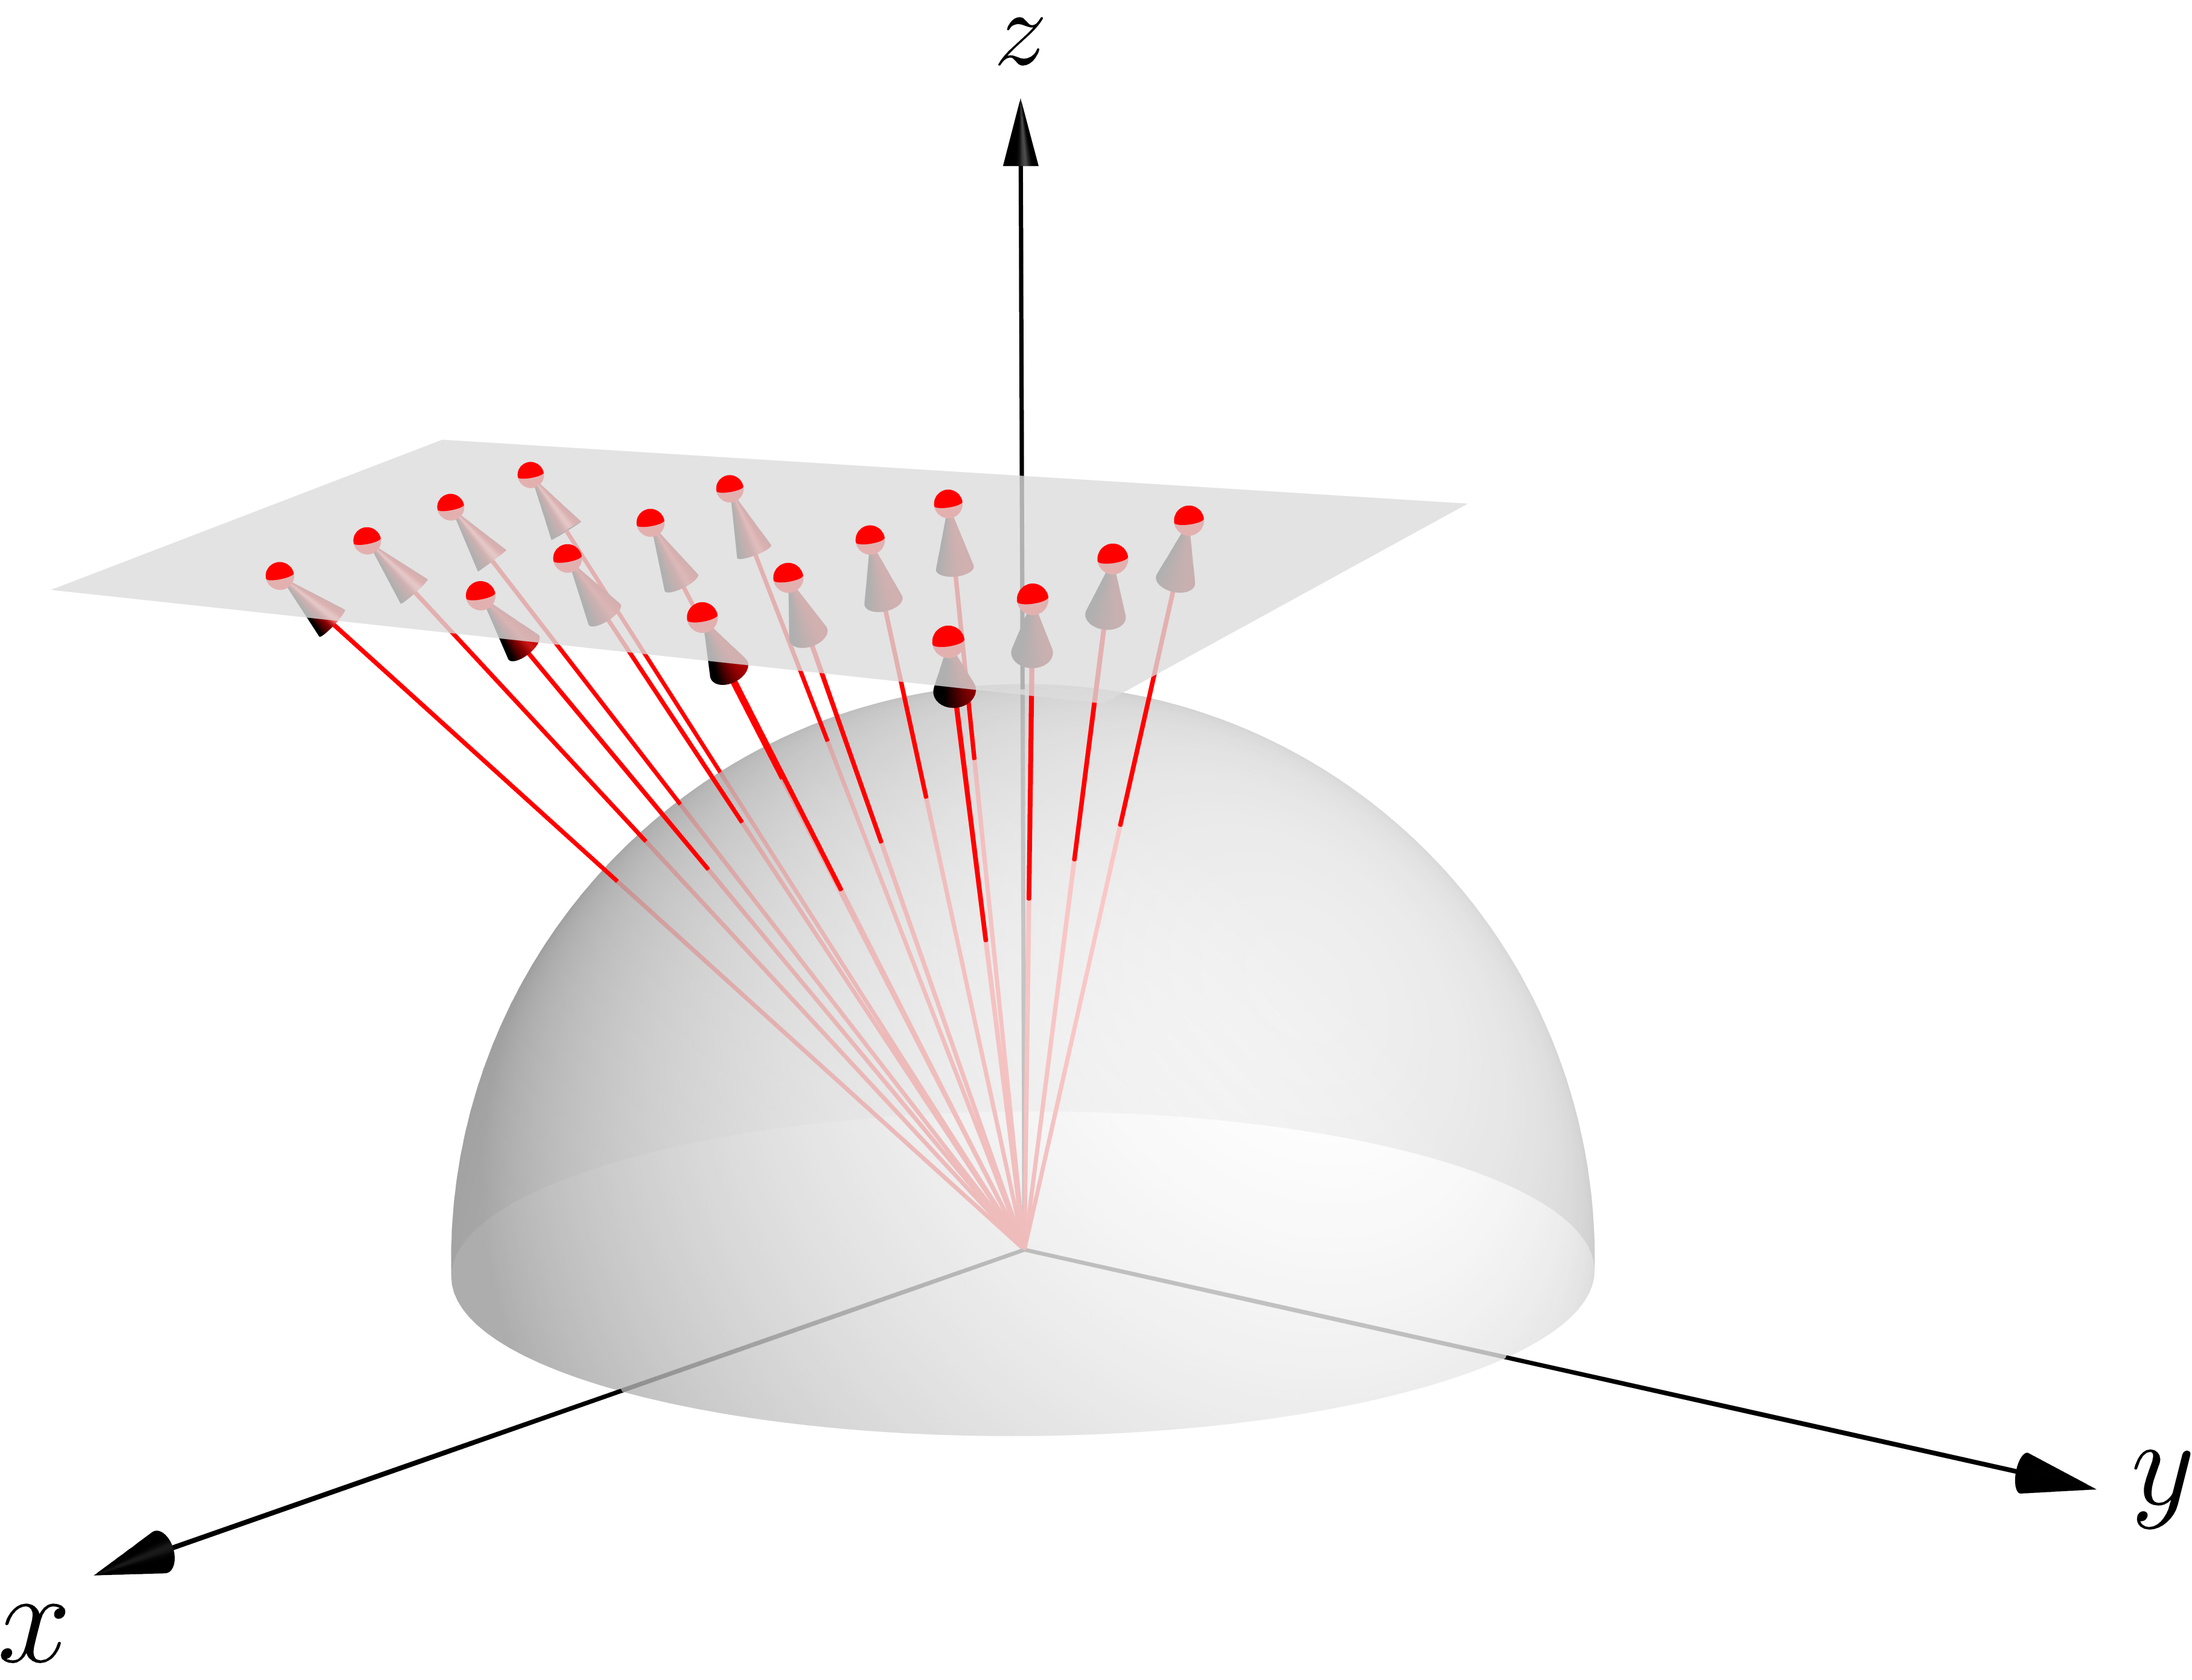
\includegraphics[width=\textwidth]{ltc/sample_transform_after}
        \label{fig:LTCTransformAfter}
        \caption{Promienie oraz wielokąt $P$ przekształcone przy użyciu $M$}
    \end{subfigure}
    
    \caption{Przekształcenie jednocześnie wielokąta i promieni powoduje, że liczba promieni przecinających wielokąt $P$ nie zmienia się. Opracowanie własne.}
    \label{fig:LTCTransformBeforeAfter}
\end{figure}

Rozumowanie można przeprowadzić na odwrót dla przekształcenia $M^{-1}$. Wynika z tego, że jeżeli będziemy w stanie znaleźć prosty rozkład bazowy, którego całkę tej postaci możemy szybko obliczyć oraz przekształcenie $M^{-1}$ przybliżające rozkład docelowy rozkładem bazowym, to wykorzystując powyższą właściwość możemy przybliżyć wartość całki rozkładu docelowego na wielokącie sferycznym.

%\begin{figure}[ht]
%\missingfigure{Obrazek kilku przekształceń rozkładu LTC}
%\end{figure}

\subsection{Wybór rozkładu bazowego $D_0(\omega)$}

Kolejnym zadaniem jest wybór rozkładu bazowego, który po przekształceniu liniowym da nam oczekiwany rozkład spełniający założenia postawione na samym początku.

Rozpocznijmy poszukiwania od najprostszego rozwiązywalnego rozkładu, a mianowicie rozkładu jednorodnego. Jeżeli rozkład $D$ przyjmuje taką samą wartość w każdym punkcie to całka na wielokącie sferycznym (ang. \textit{spherical polygon}) jest równoważna kątowi bryłowemu przemnożonym przez odpowiedni stały współczynnik, a na to istnieje wzór jawny \cite{Arvo,Snyder}. Bardzo podobnie sytuacja wygląda z półsferą z tym że, wielokąt musi zostać przycięty do horyzontu. Rozkład jednorodny opisany na półsferze możemy wyrazić wzorem:
\[
D_0(\omega_o=(x_0, y_0, z_0)) = \begin{cases}
  \frac{1}{2\pi} & \text{dla } y_0 \geq 0 \\
  0 & \text{dla } y_0 < 0
\end{cases}
\]

Niestety, oba rozkłady nie są w stanie modelować żadnych ciekawych zjawisk ze względu na niezmienną naturę.

Nieco bardziej skomplikowanym rozkładem jest przycięty rozkład kosinusowy (ang. \textit{diffuse}, \textit{Lambertian distribution}, \textit{cosine distribution}).
\[
D_0(\omega_o=(x_0, y_0, z_0)) = \begin{cases}
  \frac{y_0}{\pi} & \text{dla } y_0 \geq 0 \\
  0 & \text{dla } y_0 < 0
\end{cases}
\]

Zaletą tego rozkładu jest fakt, że przechodzi on gładko do $0$ oraz posiada prosty wzór jawny. Obliczanie całki na takim rozkładzie jest z definicji obliczaniem irradiancji wielokąta sferycznego. Istnieje wzór jawny wyprowadzony przez Lamberta \cite{Baum}:
\[
E(p_1, \ldots, p_n) =
\frac{1}{2\pi}
\sum_{i=0}^{n} {
  \cos^{-1}(\langle p_i, p_j \rangle)
  \left\langle {
    \frac{p_i \times p_j}{\norm{p_i \times p_j}},
    \left[ \begin{matrix} 0 \\ 0 \\ 1 \end{matrix} \right]
  } \right\rangle
}
\]
\[
j = (i+1) \text{ mod } n
\]

Złożoność powyższego wzoru jest liniowo zależna od stopnia złożoności wielokąta, co umożliwia zastosowanie go w aplikacjach czasu rzeczywistego.

Istnieją również inne potencjalne rozkłady bazowe, ale niestety w większości przypadków nie nadają się one do tego zastosowania. Rozkłady opisywane przez sferyczne gaussowskie (ang. \textit{spherical gaussian}) nie posiadają wzoru jawnego, rozkład Phong’a posiada wzór jawny, jednak zmienna złożoność zależna liniowo od wykładnika sprawia, że metoda jest niepraktyczna.

Z powyższych rozważań, wynika, że przycięty rozkład kosinusowy jest dobrym kandydatem na rozkład bazowy – gładko przechodzi do 0 oraz posiada prosty wzór jawny.

\section{Uwzględnienie  normy BRDF i współczynnika Fresnela}

Warto również zauważyć, że wszystkie powyższe rozkłady podstawowe mają postać znormalizowaną tzn. zachodzi warunek:
\[
\int_\Omega {
    D_0(\omega_0)
    d \omega_0
} = 1
\]

W takim przypadku istotną obserwacją jest to, że jeżeli dany materiał pochłania dużą część energii w trakcie odbicia, zastosowanie tej metody w sposób bezpośredni znając macierz przekształcającą $M$ oraz rozkład $D$ nie wystarczy \cite{LTCFresnelApprox}. Ze względu na zjawiska geometryczne wspomniane w poprzednich rozdziałach może okazać się, że:
\[
    n_D = \int_{\Omega} {
        f_r(\omega_i, \omega_o) \cos\theta_i 
        \dd \omega_i
    } \leq 1
\]
W takim przypadku konieczne jest zachowanie wartości $n_D$ razem z dopasowaniem tak, abyśmy mogli przeskalować odpowiedź $D$, tak aby była proporcjonalna do powyższego wyrażenia podcałkowego.

W wielu modelach występuje również współczynnik Fresnela, najczęściej sterowany parametrem materiałowym $F_0$. W takim przypadku, chcielibyśmy uzależnić normę skalującą wartość maksymalną całki rozkładu również od $F_0$. W tym celu skorzystamy z aproksymacji Schlicka:
\begin{gather*}
\int_{\Omega} {
    F(\omega_i, \omega_o)
    f_r(\omega_i, \omega_o) 
    \cos\theta_i 
    \dd \omega_i
} =
\int_{\Omega} {
    \left[
        F_0 + (1-F_0)(1 - \omega_v \cdot m)^5
    \right]
    f_r(\omega_i, \omega_o) 
    \cos\theta_i 
    \dd \omega_i
} = \\
= F_0 \int_{\Omega} {
    f_r(\omega_i, \omega_o) 
    \cos\theta_i 
    \dd \omega_i
} + (1-F_0) \int_{\Omega} {
    (1 - \omega_v \cdot m)^5
    f_r(\omega_i, \omega_o) 
    \cos\theta_i 
    \dd \omega_i
}
\end{gather*}

Oznaczmy:
\[
    f_D = \int_{\Omega} {
        (1 - \omega_v \cdot m)^5
        f_r(\omega_i, \omega_o) 
        \cos\theta_i 
        \dd \omega_i
    }
\]

\noindent Podstawiając za całki odpowiednio $n_D$ oraz $f_D$ otrzymamy normę postaci:
\[
    F_0 n_D + (1-F_0) f_D
\]

Stałe $n_D$ oraz $f_D$ powinny zostać wyznaczone podczas szukania optymalnej macierzy $M$ i zapisane razem z nią.


\section{Wybór przekształcenia liniowego}

Pozostaje wybór przekształcenia liniowego, którego będziemy używać do formowania naszego przybliżenia. Dla materiału izotropowego funkcja BRDF zależy tylko i wyłącznie od kąta obserwacji, zatem wektora $V = (\sin\theta, 0, \cos\theta)$ oraz współczynnika chropowatości $\alpha$.

Wróćmy znów do efektów które chcemy wymodelować. Pierwszym, najprostszym z nich jest kontrola chropowatości za pomocą współczynnika $\alpha$, która może zostać zrealizowana poprzez skalowanie niejednorodne próbek (jednorodne w płaszczyźnie $XY$, rys. \ref{fig:LTCEqualScale}):
\[
M_{\alpha} =
\begin{bmatrix}
  \lambda & 0 & 0 \\
  0 & \lambda & 0 \\
  0 & 0 & 1
\end{bmatrix}
\]

\begin{figure}[h]
\centering
    \begin{subfigure}[t]{0.25\textwidth}
        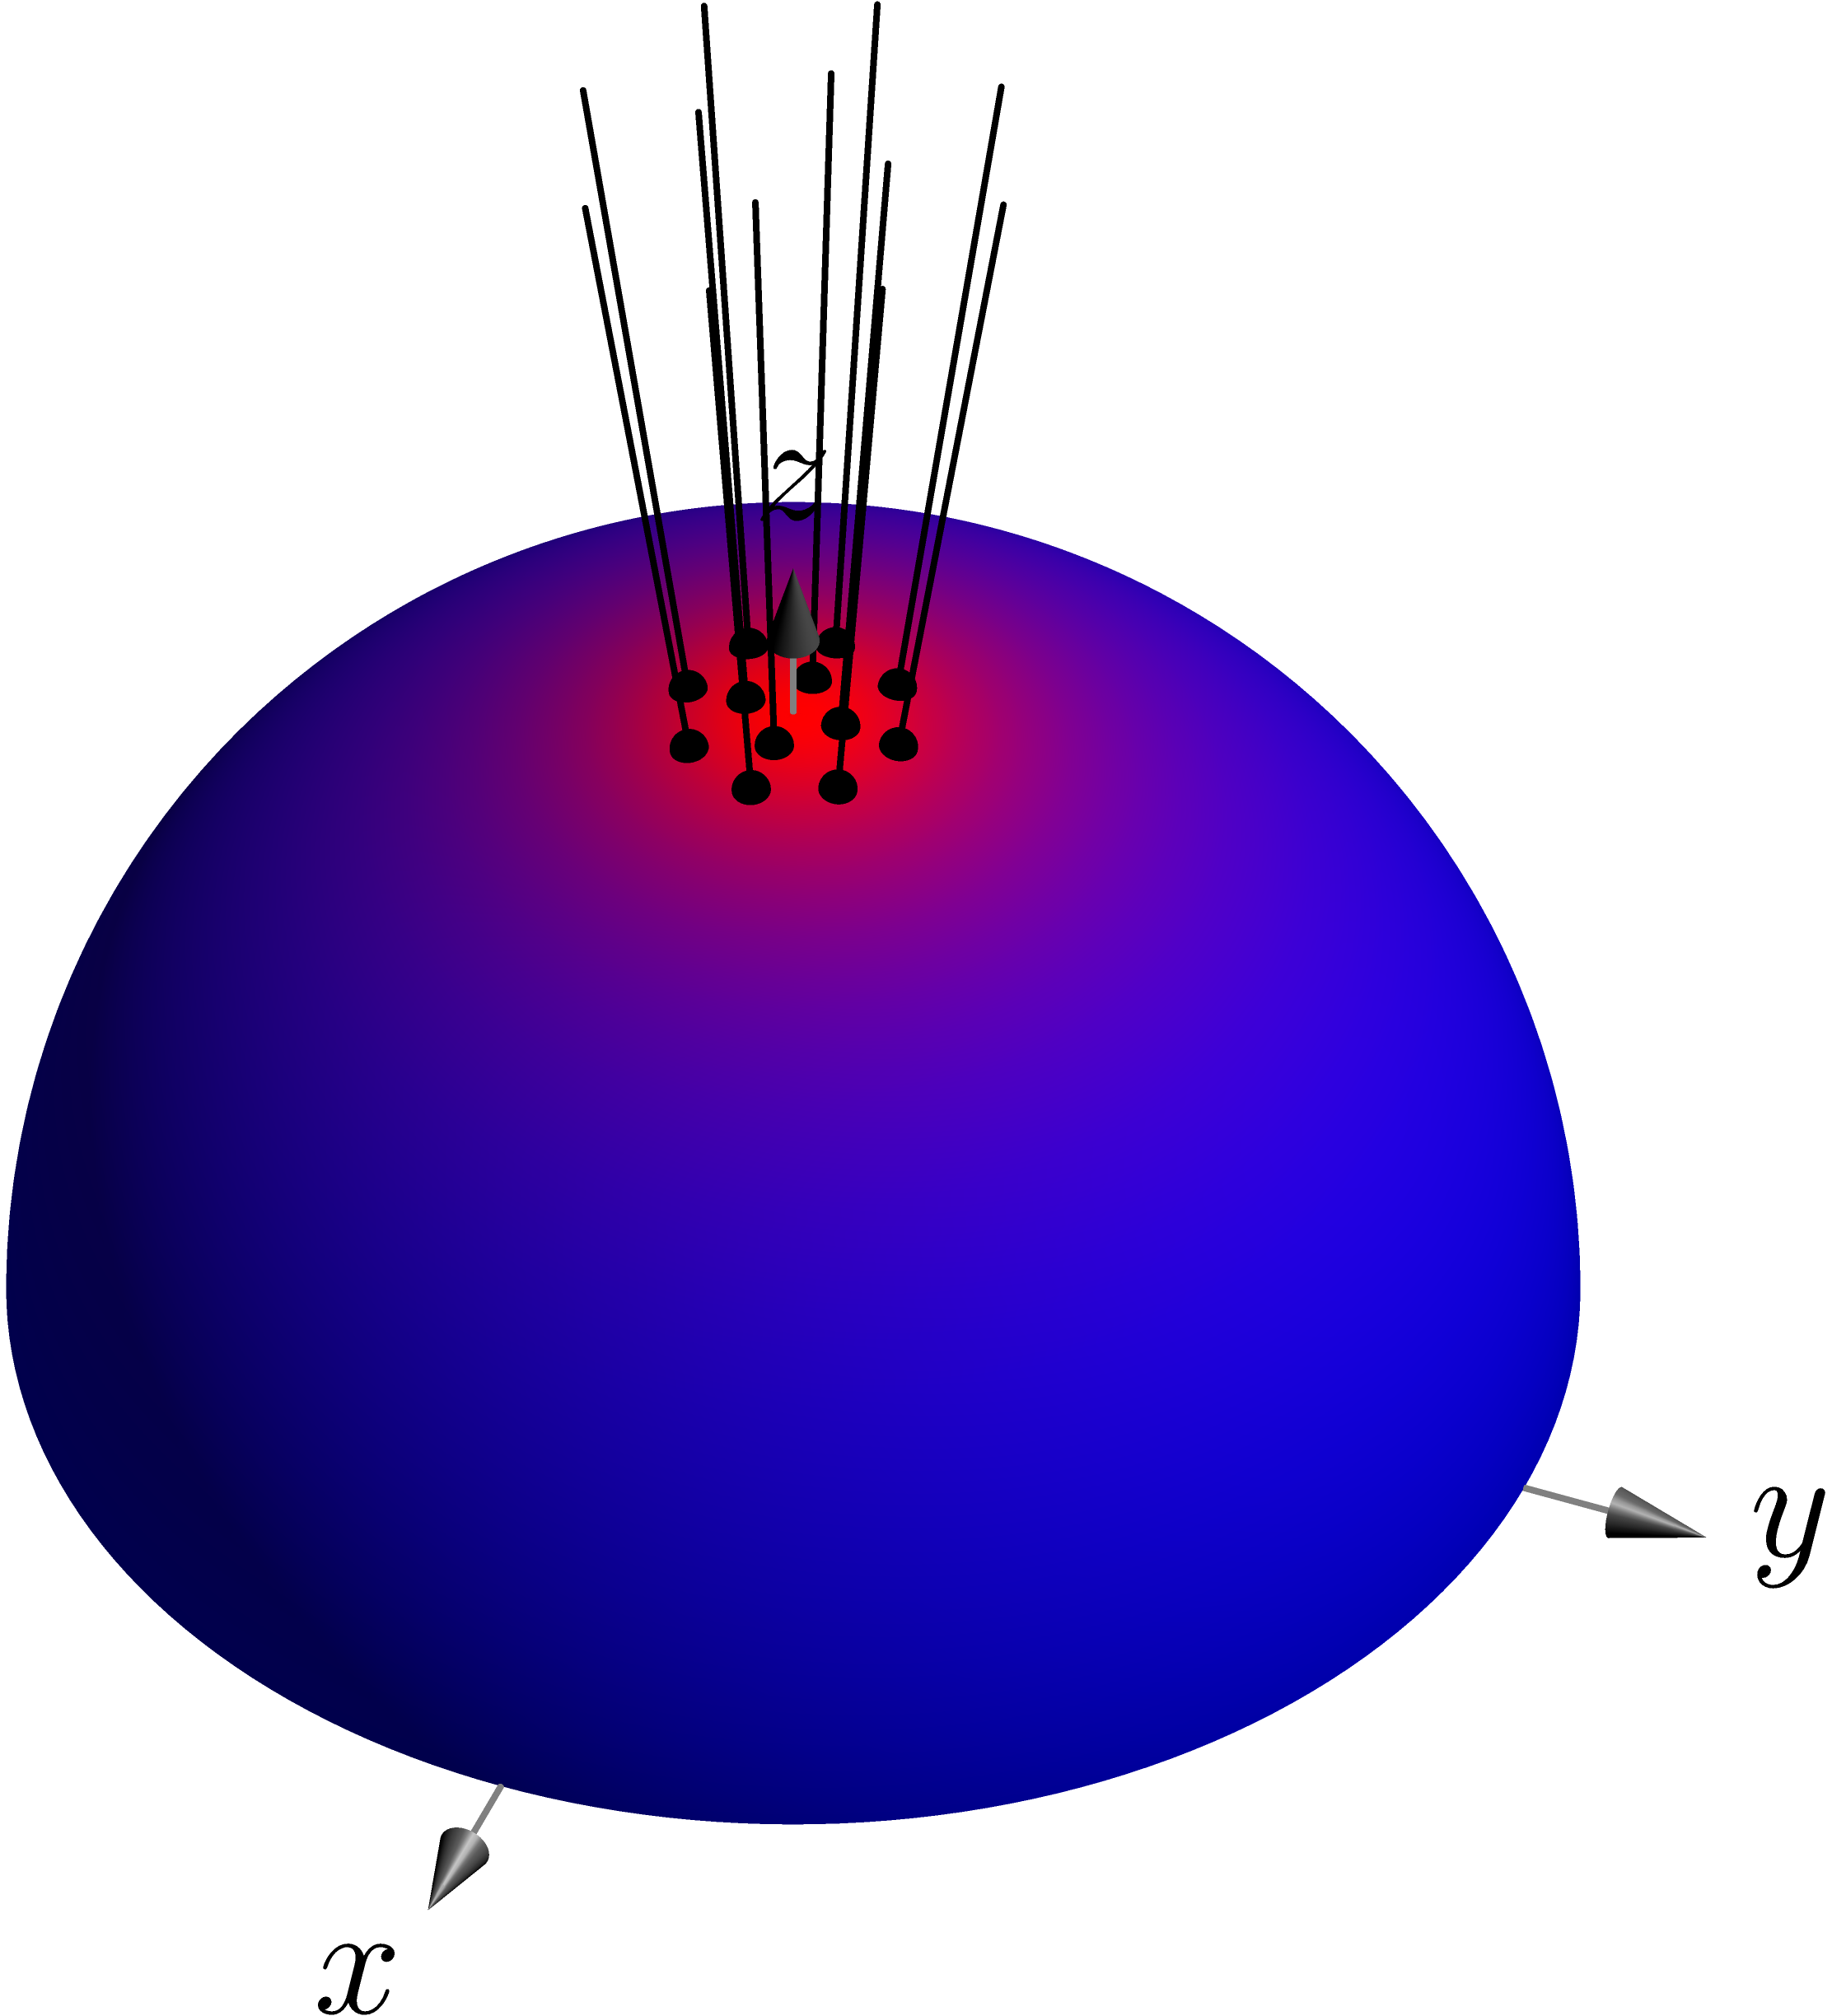
\includegraphics[height=5cm]{ltc/cosine_dist_scale.png}
        \caption{Skalowanie jednorodne.}
        \label{fig:LTCEqualScale}
    \end{subfigure}
    \hspace{0.03\textwidth}
    \begin{subfigure}[t]{0.25\textwidth}
        \centering
        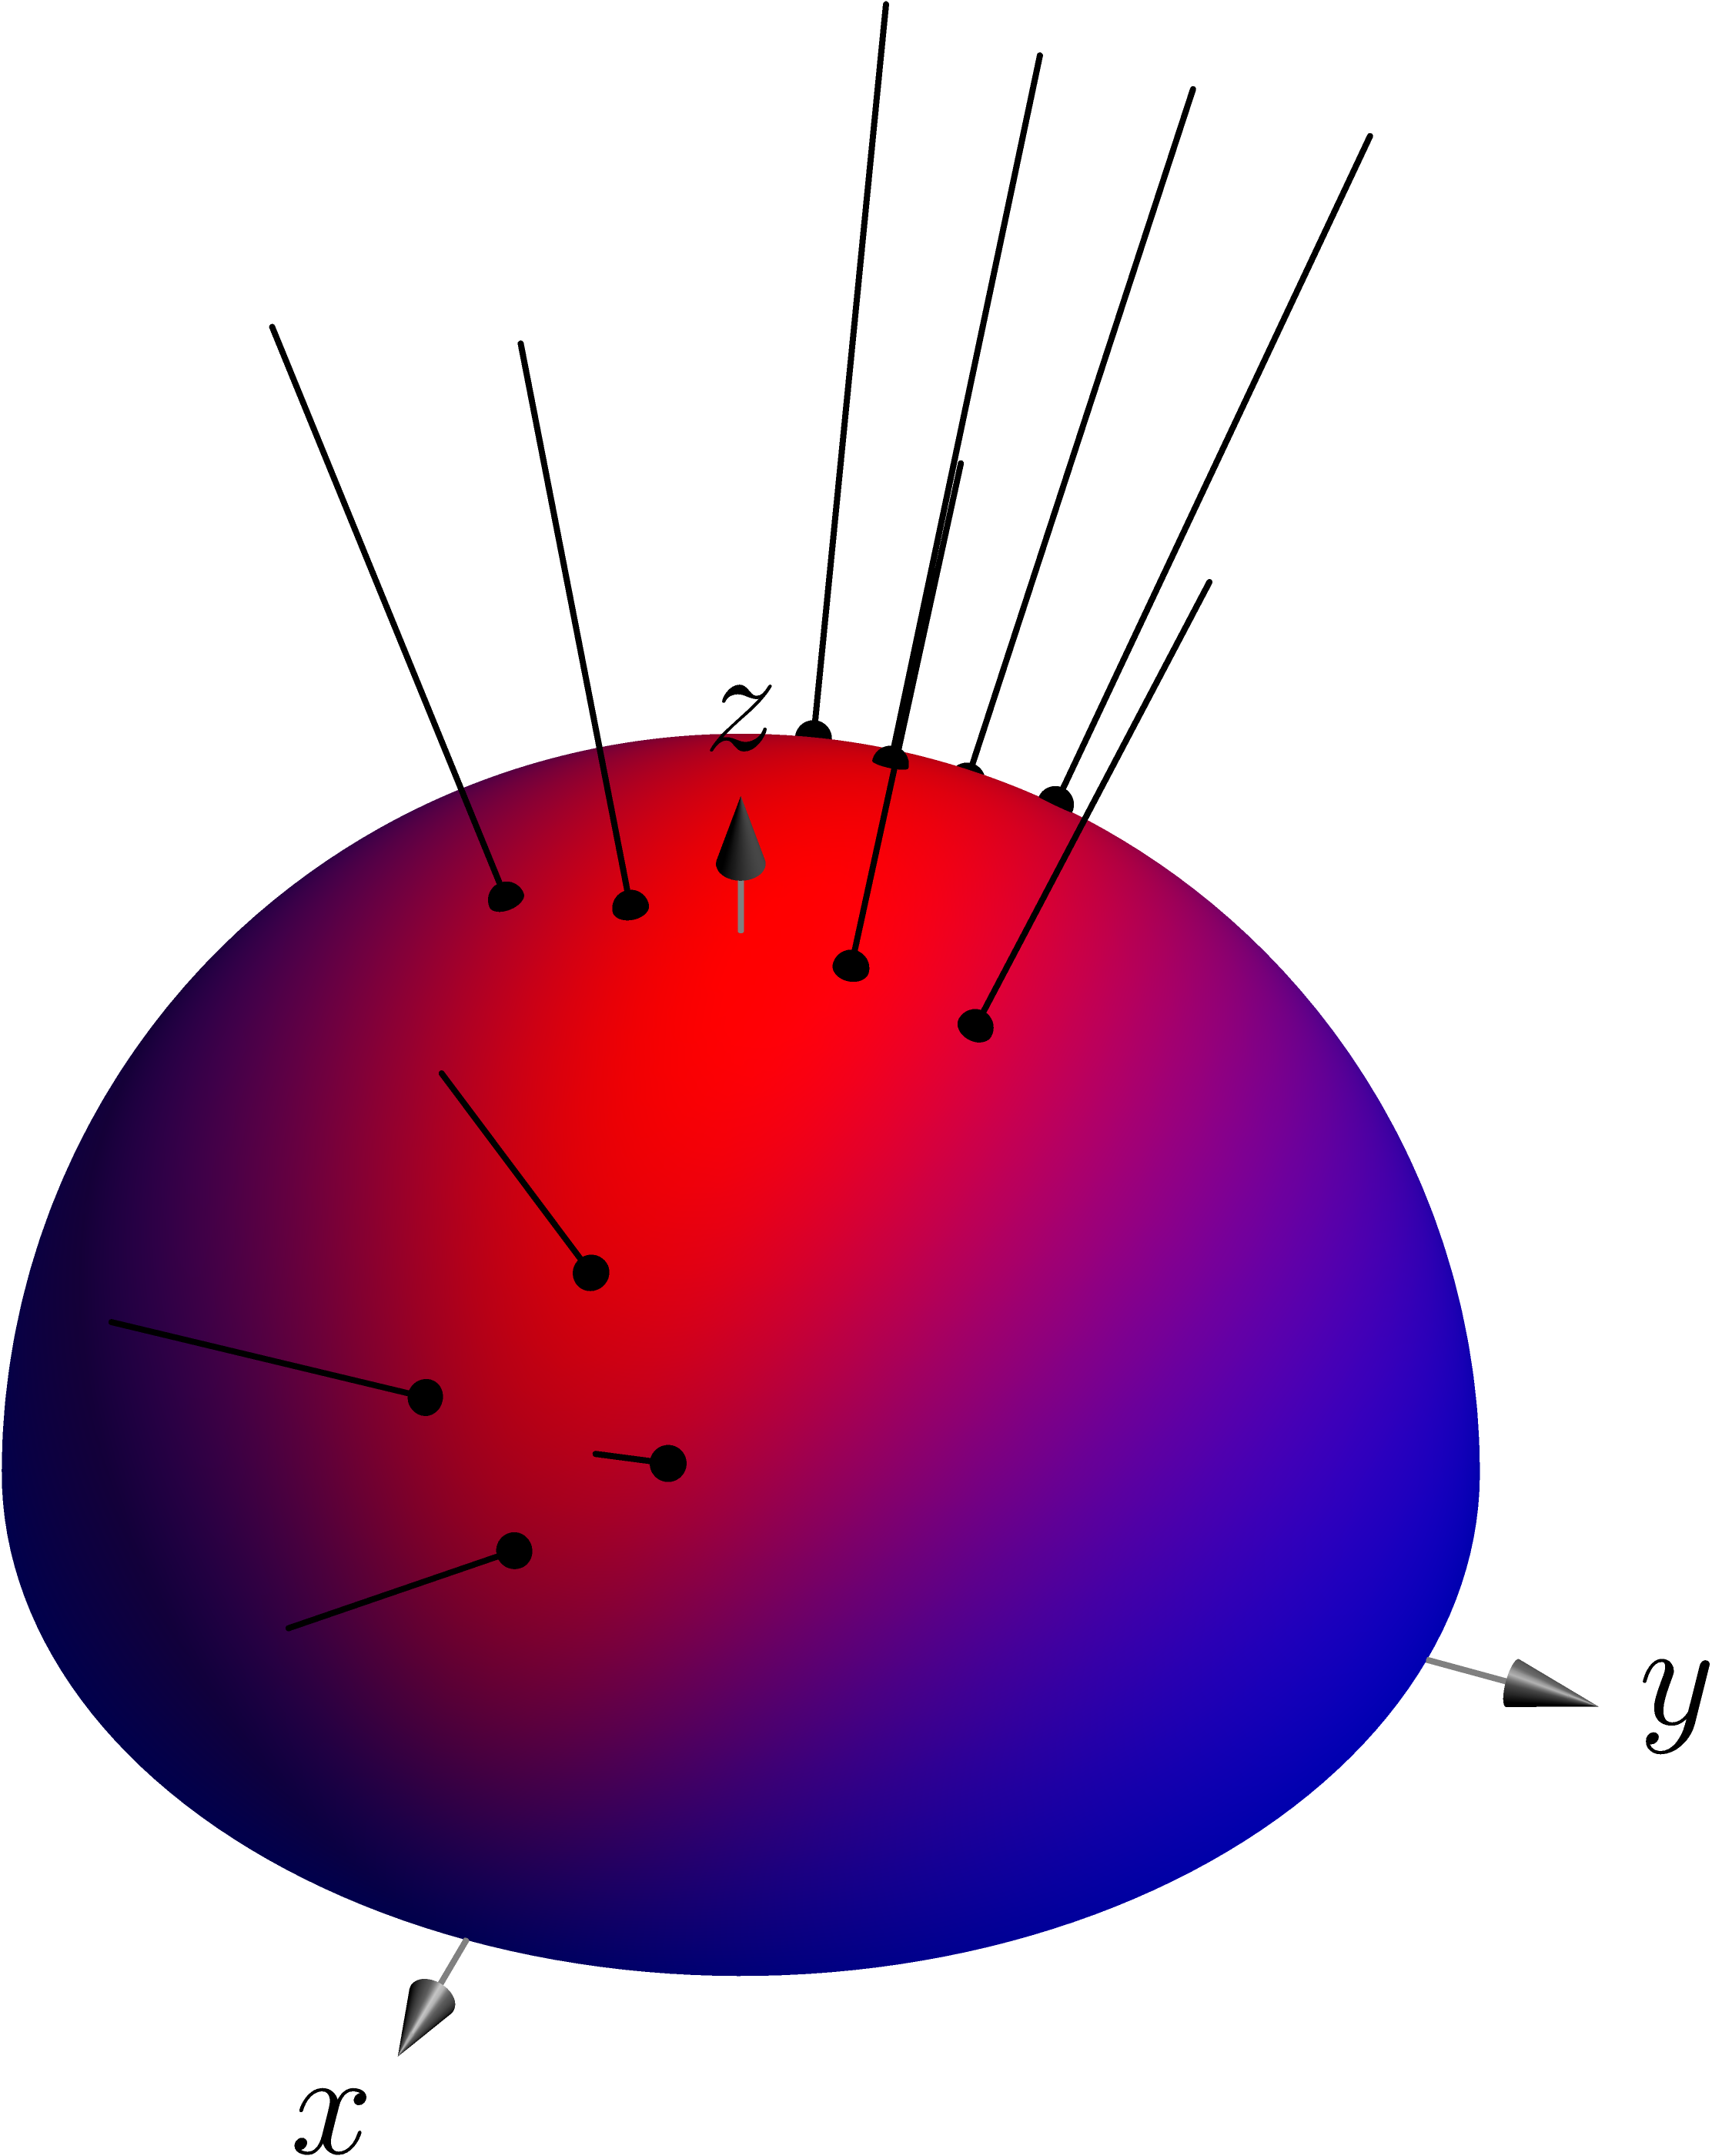
\includegraphics[height=5cm]{ltc/cosine_dist_scale_aniso.png}
        \caption{Skalowanie niejednorodne.}
        \label{fig:LTCAnisoScale}
    \end{subfigure}
    \hspace{0.03\textwidth}
    \begin{subfigure}[t]{0.25\textwidth}
        \centering
        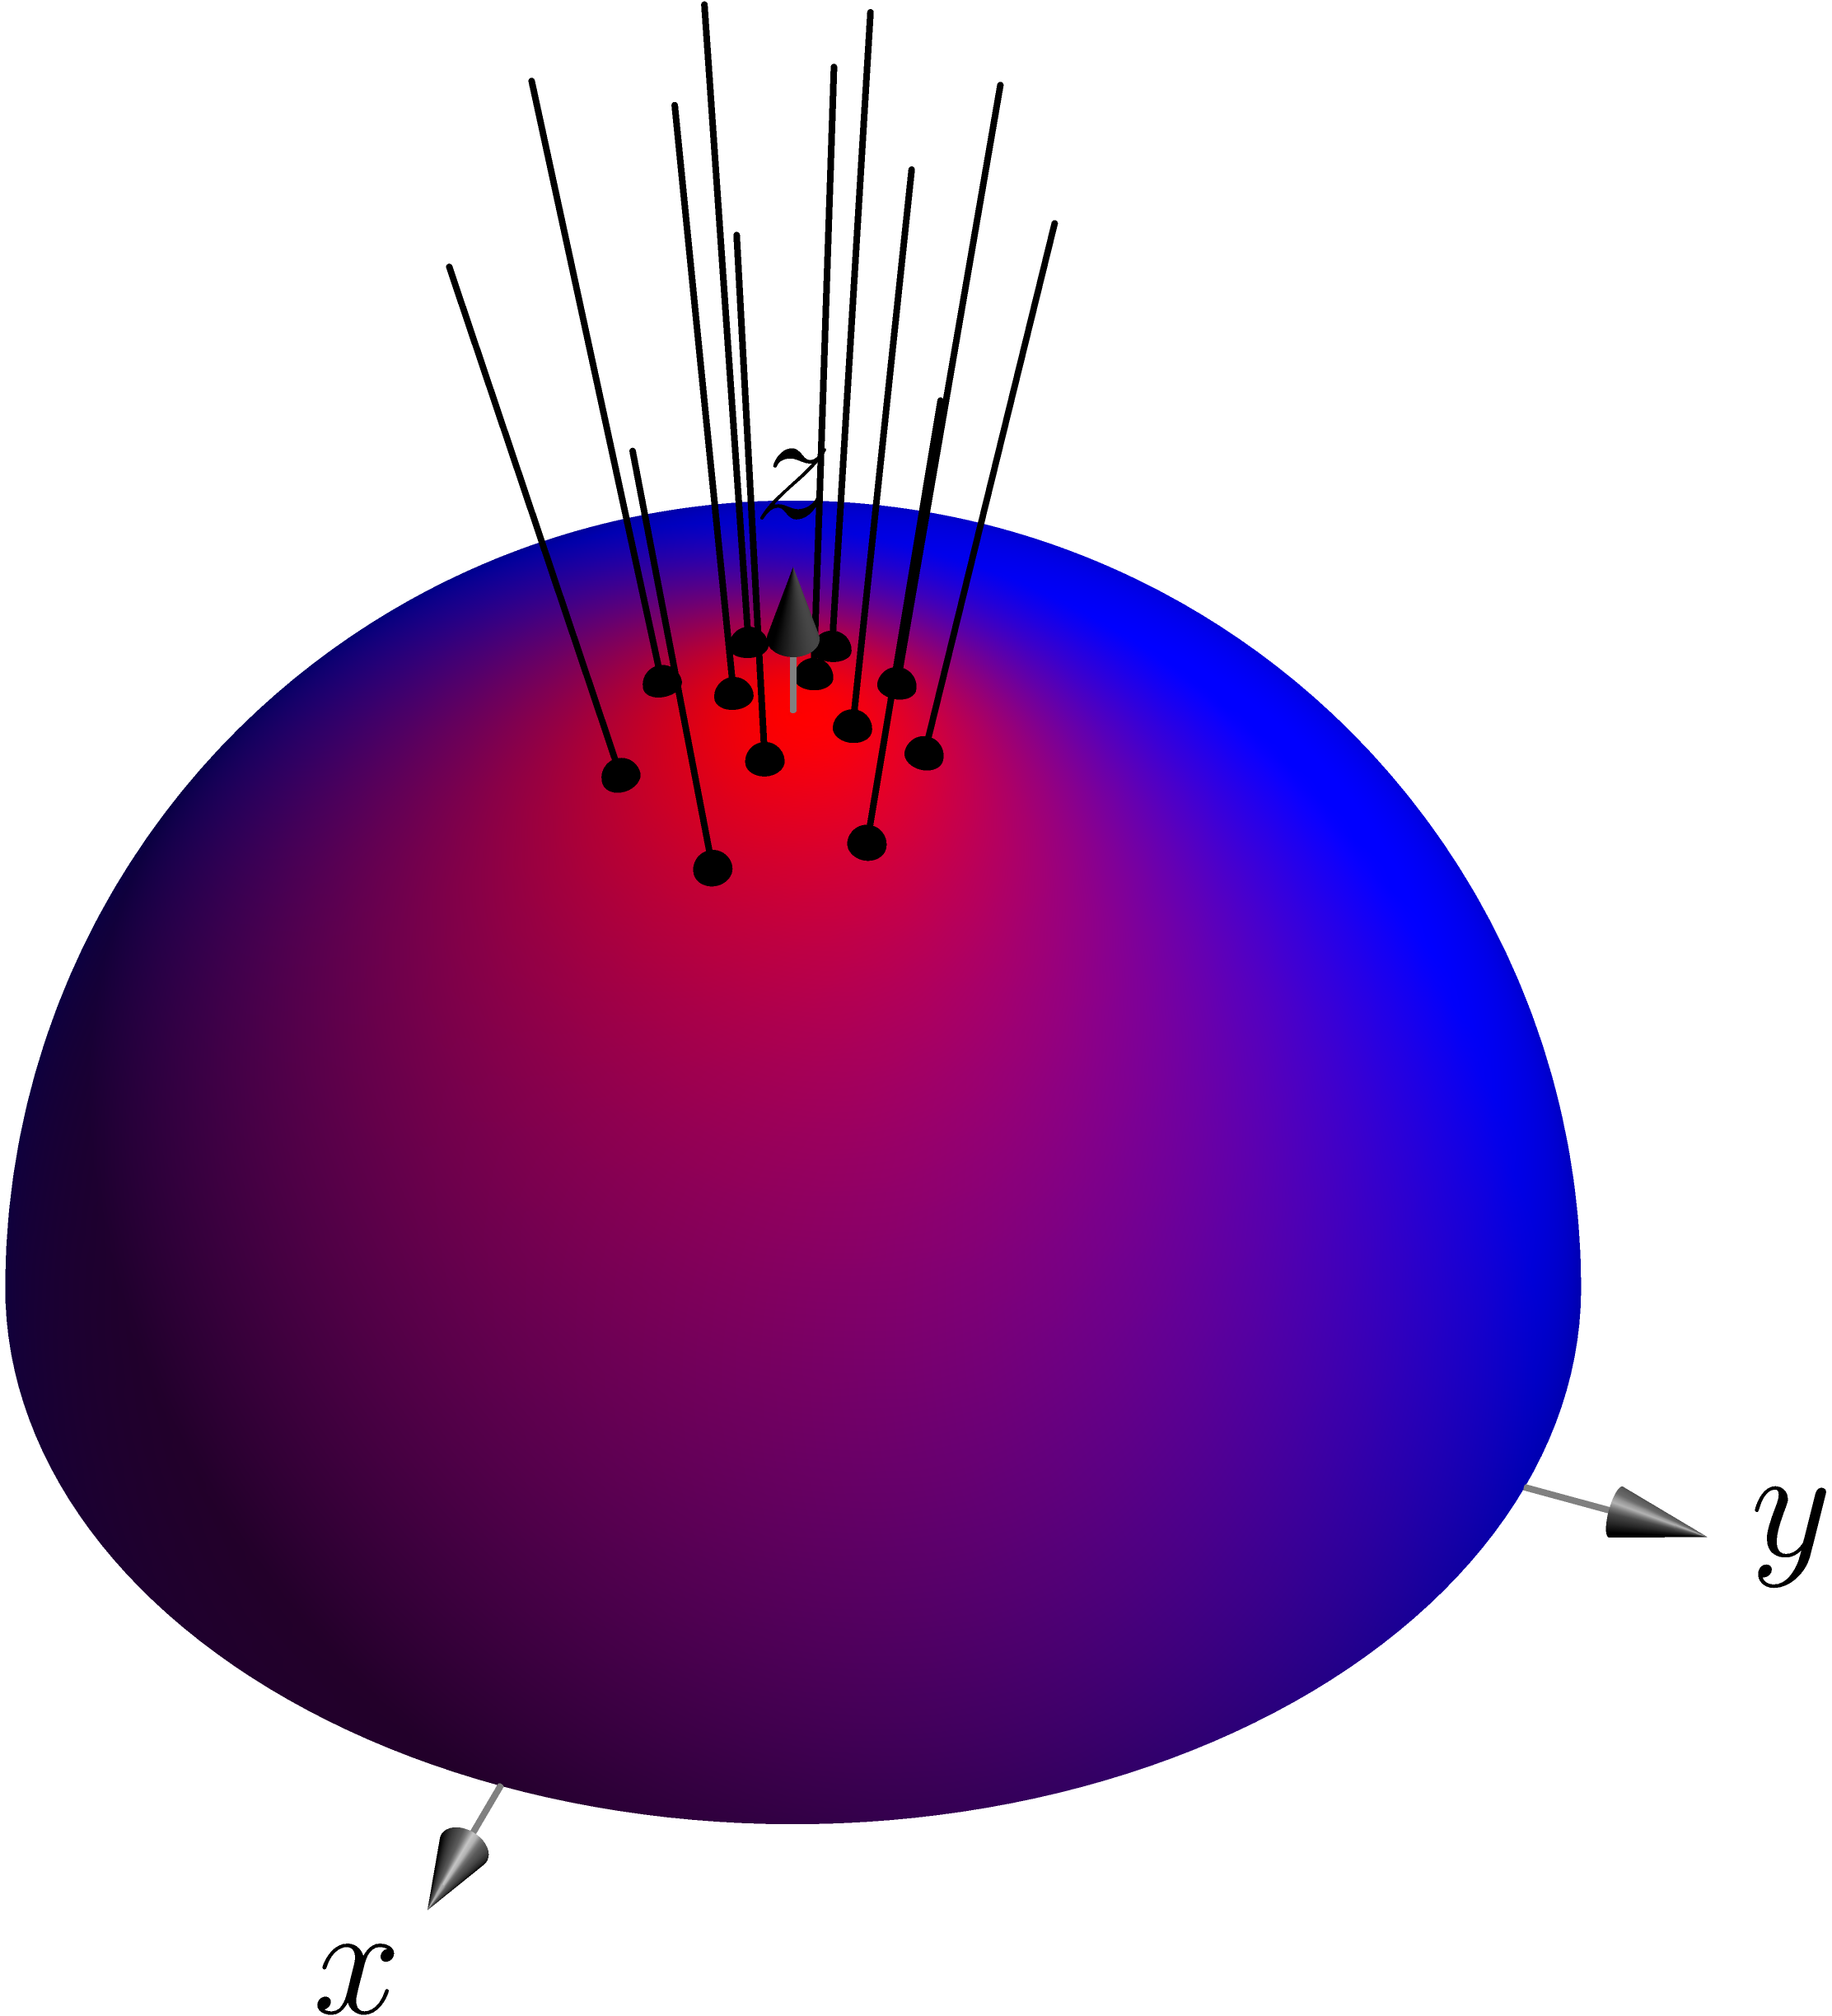
\includegraphics[height=5cm]{ltc/cosine_dist_skew.png}
        \caption{Przekształcenie skośne.}
        \label{fig:LTCSkew}
    \end{subfigure}
    \caption{Przekształcenia bazowe wykorzystane do przybliżania dowolnego rozkładu rozkładem lambertowskim. Opracowanie własne.}
    \label{fig:LTCTransforms}
\end{figure}

Anizotropia powstająca w przy dużych kątach obserwacji może zostać zasymulowana poprzez skalowanie niejednorodne w płaszczyźnie $XY$ (rys. \ref{fig:LTCAnisoScale}):
\[
M_{\text{aniso}} =
\begin{bmatrix}
  \lambda_x & 0 & 0 \\
  0 & \lambda_y & 0 \\
  0 & 0 & 1
\end{bmatrix}
\]



Zjawisko maksimum poza kątem odbicia przy rosnącej chropowatości może zostać zasymulowane poprzez skorzystanie z macierzy skośnej (rys. \ref{fig:LTCSkew}):
\[
M_{\text{skew}} =
\begin{bmatrix}
  1 & 0 & 0 \\
  0 & 1 & 0 \\
  \lambda_{s} & 0 & 1
\end{bmatrix}
\]

Powyższe przekształcenia dają nam możliwość precyzyjnego modelowania spójnych rozkładów o prostych, ale wystarczających do naszych zastosowań kształtach. Chcielibśmy teraz znaleźć przekształcenie dla danego kąta i współczynnika $\alpha$, tak, aby w rezultacie dostać przybliżenie fizycznie poprawnego rozkładu, np. rozkładu GGX (Torrance-Reitz). Po złożeniu tych macierzy otrzymujemy:

\[
M_{\text{precise}} =
\begin{bmatrix}
1 & 0 & \lambda_{\text{skew}} \\
0 & 1 & 0 \\
0 & 0 & 1
\end{bmatrix}
\begin{bmatrix}
\lambda_x & 0 & 0 \\
0 & \lambda_y & 0 \\
0 & 0 & 1
\end{bmatrix}
\begin{bmatrix}
\lambda & 0 & 0 \\
0 & \lambda & 0 \\
0 & 0 & 1
\end{bmatrix}
=
\begin{bmatrix}
\lambda\lambda_x & 0 & \lambda_{\text{skew}} \\
0 & \lambda\lambda_y & 0 \\
0 & 0 & 1
\end{bmatrix}
\stackrel{\text{ozn.}}{=}
\begin{bmatrix}
a & 0 & c \\
0 & b & 0 \\
0 & 0 & 1
\end{bmatrix}
\]

Ostatnią operacją, którą potrzebujemy do precyzyjnego dopasowania rozkładu jest rotacja, pozwalająca nam na dokładne ułożenie uformowanego rozkładu, tak, aby pokryć kierunki o najwyższej wartości (kierunki dominujące). 
\[
M_{\text{rot}} =
\begin{bmatrix}
\cos\theta  & 0     & \sin\theta \\
0           & 1     & 0 \\
-\sin\theta & 0     & \cos\theta
\end{bmatrix}
\]

Zatem finalna macierz $M$ ma postać:
\[
M = M_{\text{rot}} M_{\text{precise}} = \begin{bmatrix}
a\cos\theta & 0 & c\cos\theta + \sin\theta \\
0 & b & 0 \\
-a\sin\theta & 0 & \cos\theta - c \sin\theta
\end{bmatrix} = \begin{bmatrix}
m_{11} & 0 & m_{31} \\
0 & m_{22} & 0 \\
m_{13} & 0 & m_{33}
\end{bmatrix}
\]

Macierz $M$ zawiera cztery niewiadome $a$, $b$, $c$, $\theta$, które będziemy wyznaczać metodami numerycznymi. Wykorzystamy technikę dopasowywania danych przeprowadzoną jednokrotnie w formie przetwarzania wstępnego i wykorzystamy gotowe rezultaty podczas rysowania sceny.

Dokument \cite{ltc_heitz} sugeruje znormalizowanie macierzy tak aby $m_{33}=1$, ale powoduje to problemy z interpolacją między poszczególnymi przekształceniami w stanach pośrednich, w prezentacji \cite{LTCJourneyPresentation} można znaleźć wyjaśnienie i przykłady problemów niesionych przez te rozwiązanie.

Macierz $M$ ze specyfiki metody musi być odwracalna, zatem: $\det M \neq 0 \Rightarrow ab \neq 0$. Wprowadzimy dodatkowe założenie, że parametry $a$ i $b$ są dodatnie, ze względu na to, że ujemny parametr będzie oznaczał odbicie lustrzane względem osi. W ten sposób również zagwarantujemy sobie poprawność znalezionego rozwiązania.

\section{Dopasowywanie rozkładu}

W celu dopasowania przekształcenia liniowego dla danych $\alpha$ i $\theta$ wykorzystamy algorytm optymalizacji numerycznej.

W celu przyśpieszenia dopasowywania znajdziemy najpierw kierunek dominujący:
\[ 
    \omega_d = \left(\sin\theta, 0, \cos\theta\right) 
\]
\noindent oraz normę $n_D$ i $f_D$ przybliżanego rozkładu rozkładu. Dane te umożliwią nam wstępne ustawienie rozkładu bazowego tak, aby najważniejsze kierunki tych rozkładów pokryły się. Informacje te są możliwe do wyprowadzenia korzystając z metody Monte Carlo z ważeniem próbek, opisanym przez poniższe równania:
\[
n_D = \int_{\Omega} D_{\text{BRDF}}(\omega)d\omega
\stackrel{n \rightarrow \infty}{=}
\frac{1}{n} \sum_{i=1}^{n} {
  \frac{
    D_{\text{BRDF}}(\omega_i)
  }{
    \text{pdf}_{\text{BRDF}}(\omega_i)
  }
}
\]
\[
f_D = \int_{\Omega} D_{\text{BRDF}}(\omega)d\omega
\stackrel{n \rightarrow \infty}{=}
\frac{1}{n} \sum_{i=1}^{n} {
    \frac{
        D_{\text{BRDF}}(\omega_i) (1 - \omega_i \cdot h)^5
    }{
        \text{pdf}_{\text{BRDF}}(\omega_i)
    }
}
\]
\[
\omega_d
\stackrel{n \rightarrow \infty}{=}
\frac{1}{n} \sum_{i=1}^{n} {
  \frac{
    D_{\text{BRDF}}(\omega_i)
  }{
    \text{pdf}_{\text{BRDF}}(\omega_i)
  }
  \omega_i
}
\]

W przypadku anizotropowym chcielibyśmy przeprowadzać obliczenia w pewnej płaszczyźnie ze względu na uproszczenie obliczeń, w naszym przypadku założyliśmy że $y(\omega_d)=0$ dla kierunku obserwacji.  Obliczenie kierunku $\omega_d$ metodą Monte-Carlo może spowodować zajście sprzecznego warunku $y(\omega_d) \neq 0$. Dlatego też dokonujemy przyciągnięcia wektora do płaszczyzny XZ:
\[
\widetilde{\omega}_d = \frac{
    \left( \omega_x,0,\omega_z \right)
  }{
    w_x^2+w_z^2
  }
\]

Kolejnym krokiem jest ustawienie ,,czubka'' rozkładu kosinusowego w kierunku dominującym $\omega_d$, czyli zbudowanie układu w którym oś $Z$ będzie pokrywać się z kierunkiem $\omega_d$. Uzyskana macierz $M_{\text{rot}}$ będzie częścią składową finalnej macierzy $M$.
\[
M_{\text{rot}} =
\begin{bmatrix}
  \cos\theta  & 0     & \sin\theta \\
  0           & 1     & 0 \\
  -\sin\theta & 0     & \cos\theta
\end{bmatrix}
= \begin{bmatrix}
  \bot {\widetilde{\omega}_d} & Y & \widetilde{\omega}_d
\end{bmatrix}
\]

Kolejnym krokiem jest ukształtowanie rozkładu do formy uwzględniającej parametry wejściowe i występujące zjawiska tj. chropowatość ($\alpha$), anizotropowość przy dużych kątach obserwacji i efekt skośny (występujący na jednej z osi), co wymaga numerycznego wyznaczenia parametrów $a$, $b$ i $c$ opisanych w poprzednim podrozdziale.

\subsection{Metoda pływającego sympleksu}

Zdefiniujmy nasz problem w postaci problemu optymalizacyjnego. Chcielibyśmy zminimalizować funkcję $f(a,b,c)$, będącą miarą różnicy (błędu) absolutnej pomiędzy oryginalnym rozkładem, a przybliżonym. Formalną definicję funkcji opiszę w kolejnym podrozdziale.

Funkcja ta posiada dwa ograniczenia narzucone przez warunek $detM \neq 0$, a mianowicie:
  $a > 0 \wedge b > 0$

Oryginalna metoda pływającego sympleksu \cite{NelderMead65} nie posiada mechanizmu dla ograniczeń, ale istnieją techniki pozwalające rozwiązać ten problem. W mojej implementacji wykorzystałem logarytmiczną wewnętrzną (barierową) funkcję kary:
\[
  p_{\mathbb{L}}(x, \rho) = - \frac{1}{\rho} \sum_{i=1}^{m} \log(-g_i(x))
\]

Alternatywną funkcją barierową jest funkcja hiperboliczna:
\[
  p_{\mathbb{H}}(x, \rho) =
    - \frac{1}{\rho} \sum_{i=1}^{m} \frac{1}{g_i(x)}
\]

\subsection{Wyznaczanie błędu przybliżenia}

Mając pewne parametry $a$, $b$, $c$ będące wynikiem kroku algorytmu optymalizacji chcielibyśmy ocenić jakość przybliżenia wyznaczonego przez te parametry. W tym celu stworzymy funkcję błędu:
\[
  f(a,b,c) =
    \int_{\Omega} {
      \abs{
        {D_{\text{LTC}}(a, b, c, \omega) - D_{\text{BRDF}}(\omega)}
      }
    } \dd \omega
\]

Funkcja ta może zostać obliczona z wykorzystaniem techniki MIS opisanej w rozdziale \ref{Chapter:MIS}.

\section{Cieniowanie sceny}

Kolor danego punktu $p$ obserwowanego pod kątem $\theta$ do normalnej, o chropowatości $\alpha$, oświetlonego światłem powierzchniowym $P$ o stałej luminancji energetycznej $L$ możemy z łatwością wyznaczyć znając już macierz $M$.

Pierwszym krokiem jest przekształcenie wielokąta $P$ transformacją $M$ oraz obcięcie go do horyzontu (rys. \ref{fig:QuadClip}). Obcinanie może być zrealizowane przez proste przejście po krawędziach i odrzucenie części dla której zachodzi $z=0$ i łącząc punkty niespójności liniami prostymi (dla tych linii składowa $z$ będzie zawsze równa $0$). Implementacja zastosowana przez \cite{ltc_heitz}, z której również korzysta ta praca, obsługuje każdy przypadek osobno ze względów wydajnościowych.

\begin{figure}[h]
    \centering
    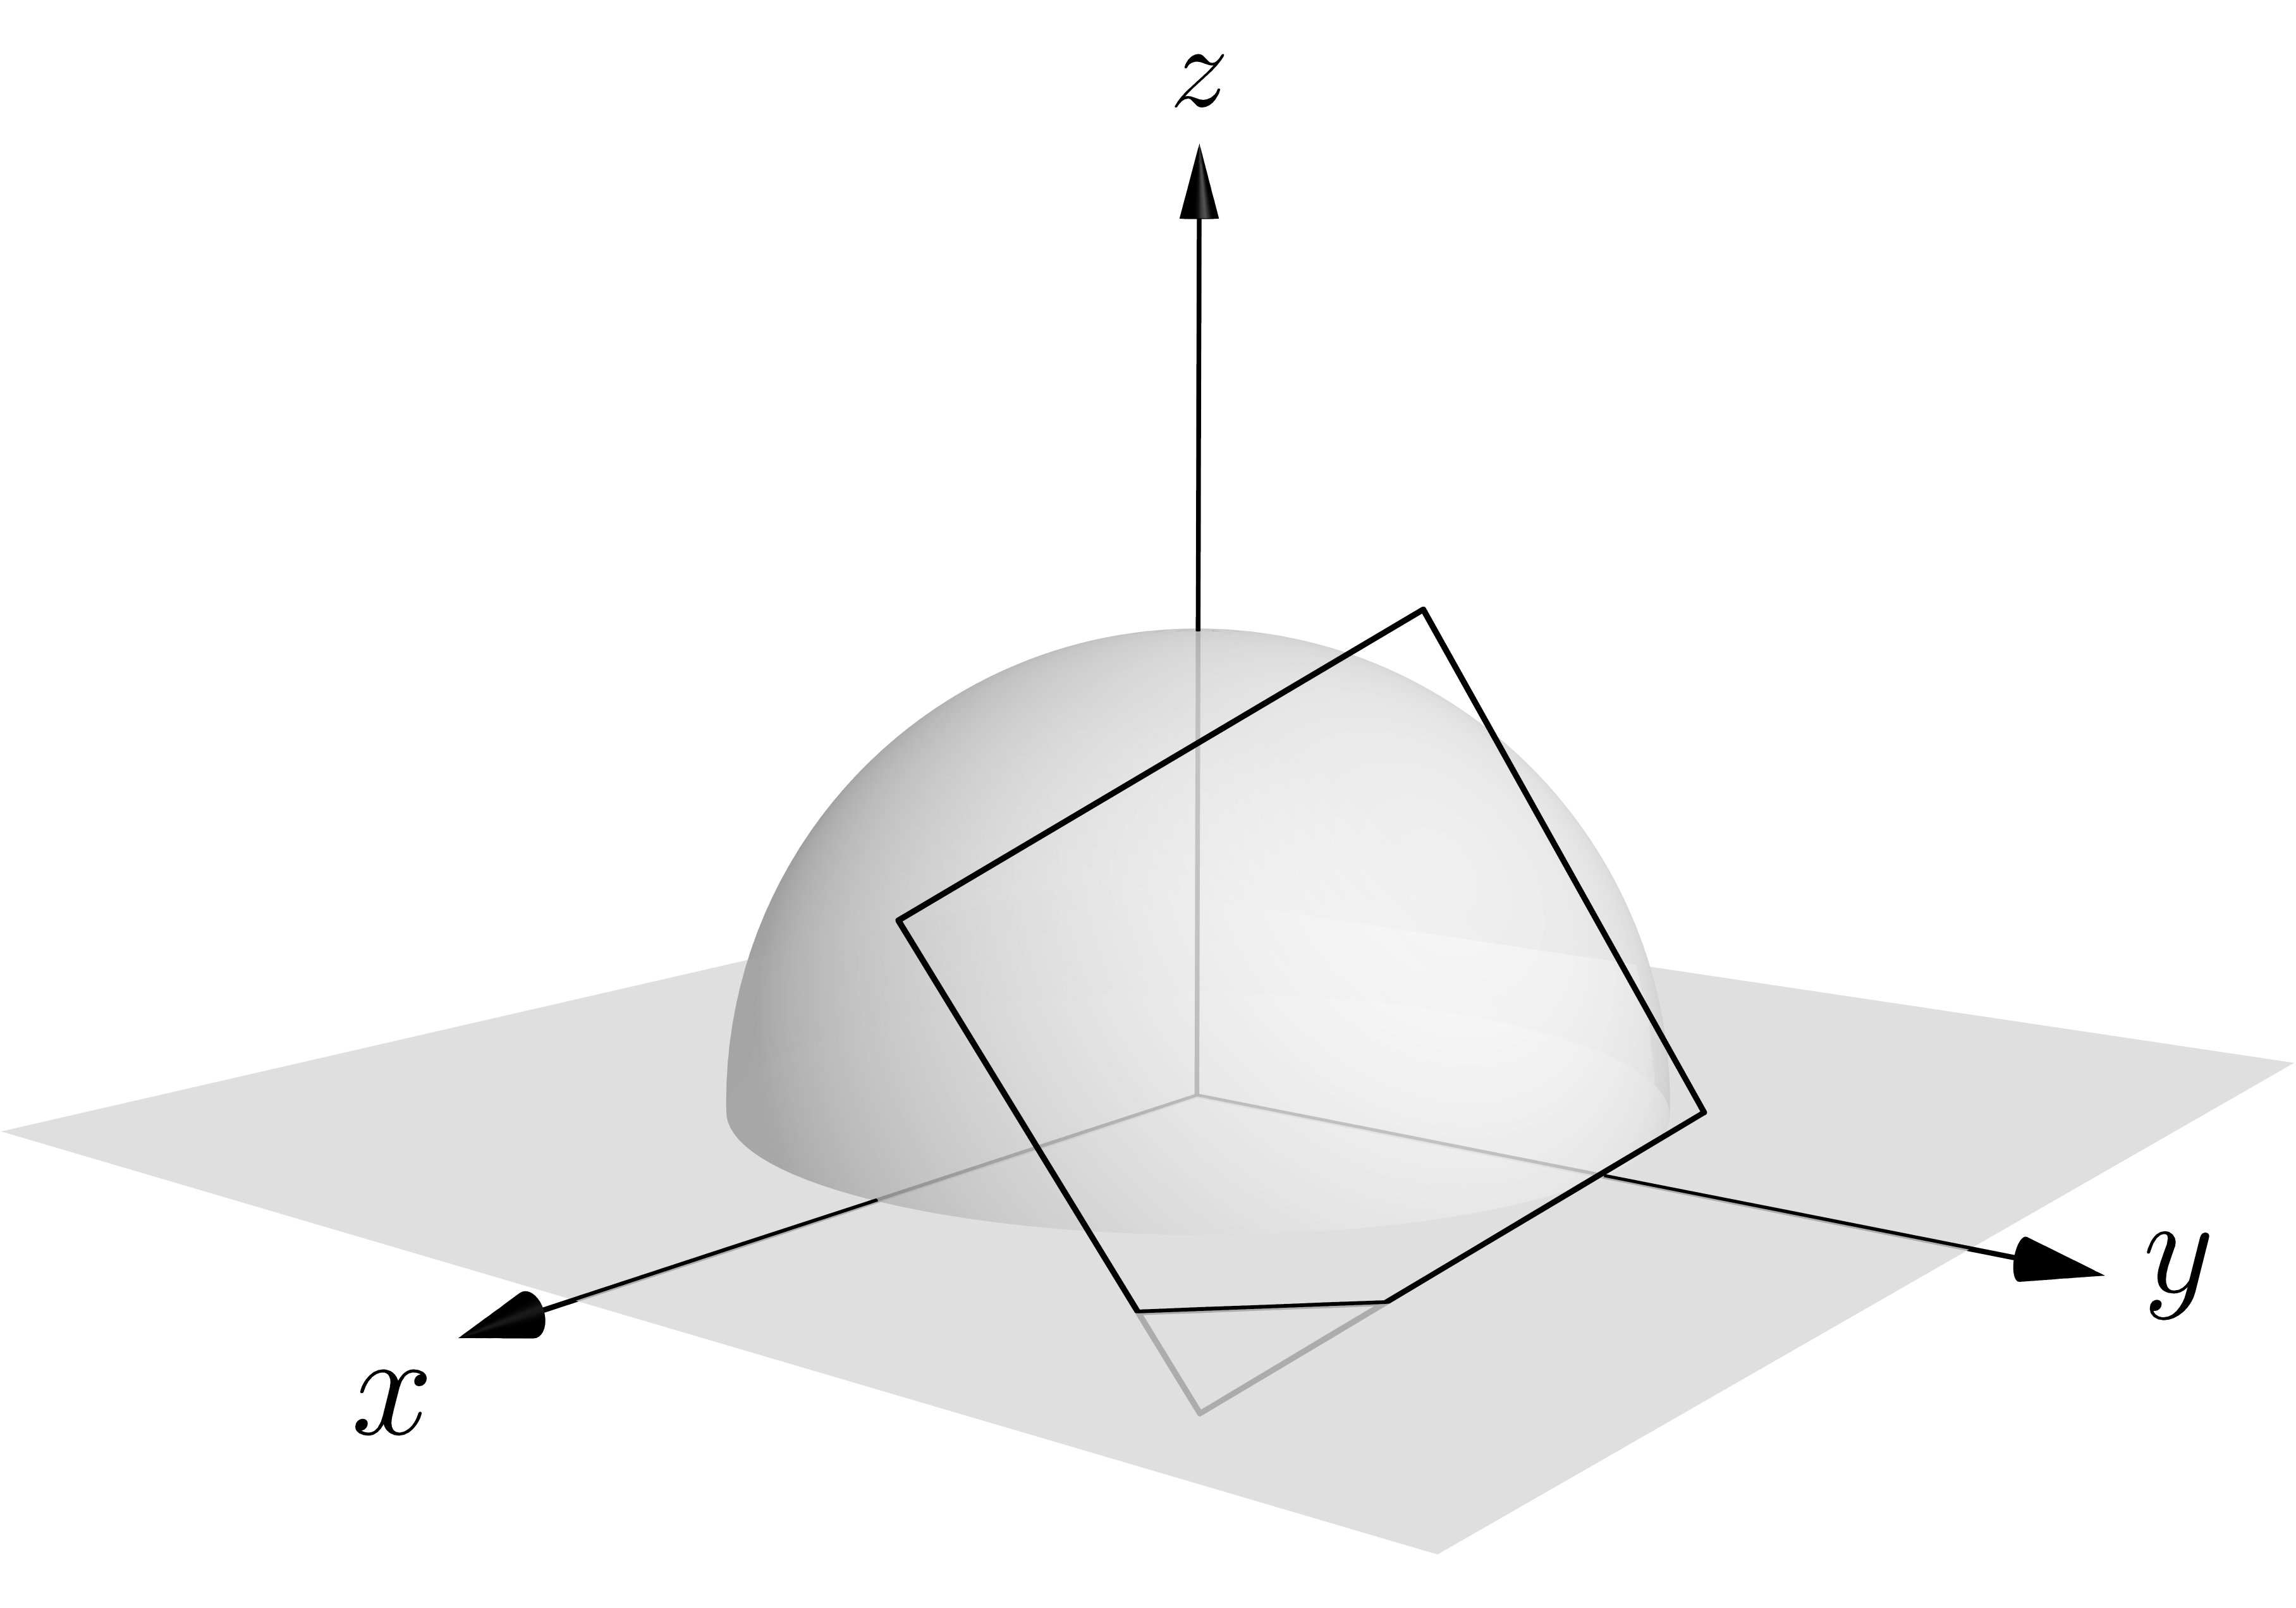
\includegraphics[width=0.6\textwidth]{ltc/quad_clip}
    \caption{Prostokątne źródło światła przycięte do horyzontu. Opracowanie własne.}
    \label{fig:QuadClip}
\end{figure}

Kolejnym krokiem jest obliczenie irradiancji tego wielokąta przy użyciu wcześniej wspomnianego wzoru wyprowadzonego przez Lamberta:
\[
E(p_1, \ldots, p_n) =
\frac{1}{2\pi}
\sum_{i=0}^{n} {
    \cos^{-1}(\langle p_i, p_j \rangle)
    \left\langle {
        \frac{p_i \times p_j}{\norm{p_i \times p_j}},
        \left[ \begin{matrix} 0 \\ 0 \\ 1 \end{matrix} \right]
    } \right\rangle
}
\]
\[
j = (i+1) \text{ mod } n
\]

Bezpośrednia implementacja powyższego wzoru niestety nie da nam oczekiwanych rezultatów, ze względu na przybliżenia zastosowane do implementacji funkcji $\cos^{-1}$ na kartach graficznych. Błąd, mimo że niewielki, jest zbyt duży do poprawnego wyznaczenia irradiancji wielokąta. W związku z powyższym autorzy \cite{LTCJourneyPresentation} proponują własne przybliżenie.

Okazuje się, że dobre rezultaty daje przybliżenie większej części równania, a mianowicie czynnika $\frac{\theta}{\sin\theta}$ \footnote{Użyteczność tej formy wynika z faktu, że $\norm{p_i \times p_j} = \norm{p_i}\:\norm{p_j}\sin\theta$.}. Metodą prób i błędów autorom udało się dobrać funkcję przybliżającą korzystając z optymalizacji funkcji. Funkcja wyznacza dobre przybliżenie dla parametru:
\[
\gamma = \abs{\cos\theta} = \abs{\langle p_i, p_j \rangle}
\]
\noindent gdy zachodzi $\cos\theta \in (0,1]$ możemy zapisać:
\[
\frac{\theta}{\sin\theta} = f(\gamma) = \frac{
    5.42031 + \left( 3.12829 + 0.0902326 \gamma \right) \gamma
}{
    3.45068 + \left( 4.18814 + \gamma \right) \gamma
}
\]
\noindent W przypadku, gdy $\cos\theta \in [-1, 0)$, możemy wyznaczyć wartość przybliżenia korzystając z własności:
\[
    \frac{\pi - \theta}{\sin\left( \pi-\theta \right)} =
    \frac{\pi - \theta}{\sin\theta} = 
    \frac{\pi}{\sqrt{1-\cos^{2}\theta}} - \frac{\theta}{\sin\theta} =
    \frac{\pi}{\sqrt{1-\gamma^2}} - f(\gamma)
\]

W zależności od tego, czy światło jest dwustronne czy nie, należy wziąć wartość absolutną irradiancji $E$ lub obciąć ją do zera. Do obliczenia końcowej wartości wykorzystujemy wzór, w którym wyprowadziliśmy czynnik Fresnelowski:
\[
    \text{spec} = E_{spec} * (F_0 n_D + (1-F_0) f_D)
\]

Pozostaje nam jeszcze obliczenie wpływu czynnika rozproszonego. Do tego wystarczy wykorzystać macierz $M=I$, ponownie obliczyć irradiancję wielokąta. 
\[
    L_o = L_i * \left( \text{spec} + c_{diff}*E_{diff} \right)
\]

\subsection{Format danych}

Ze względu na ograniczenia techniczne do zbudowania podglądu przekształceń wykorzystamy równomierną siatkę próbek $n \times n$ na kostce $(\alpha, \theta) \in \left[0,1\right] \times \left[0, \frac{\pi}{2}\right]$.

Plik zawierający wyniki dla poszczególnych $\alpha$, $\theta$ przechowuje je w formie dwóch tablic dwuwymiarowych przetworzonych w taki sposób, aby były gotowe do wczytania przez kartkę graficzną bez dodatkowych obliczeń. Dokładny opis formatu pliku znajduje się w rozdziale poświęconym architekturze aplikacji (rozdział \ref{chapter:TODO}).

Pierwsza tekstura zawiera współczynniki $M_{1}^{1}, M_{1}^{3}, M_{2}^{2}, M_{3}^{1}$ w postaci liczb zmiennoprzecinkowych o pojedynczej precyzji. Druga tekstura zawiera pozostały istotny współczynnik, czyli $M_{3}^{3}$, normę referencyjnego BRDF $n_D$ oraz oszacowany współczynnik Fresnela $f_D$.

\end{document}
